\newpage
\section{Ereignisse und ihre Wahrscheinlichkeit}

	\begin{tabular}{|l|l|c|}
		\hline
		Begriff & Beschreibung & Modell\\
		\hline
		Elementarereignis & Der Ausgang eines Experiments & $\omega$\\
		alle Elementarereignisse & Alle mögliche Ausgänge eines Experiments & $\Omega$ \\
		Ereignis & Teilmenge von $\Omega$ \quad $A$ eingetreten $\Leftrightarrow$ Versuchsausgang $\omega \in A$ \ & $A \subset \Omega$\\
		\hline
	\end{tabular}
	
	\vspace{0.2cm}
	
	\begin{tabular}{|l|l|c|c|}
		\hline
		Begriff & Beschreibung & Bild & Modell\\
		\hline
		Sicheres Ereignis & tritt immer ein & %Autor: Simon Walker
%Version: 1.0
%Datum: 25.11.2019
%Lizenz: CC BY-NC-SA

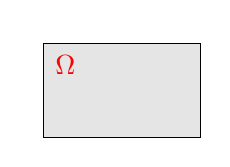
\begin{tikzpicture}[xscale=0.4, yscale=0.4]
	\fill[white, fill opacity=0] (-0.5,0) rectangle (5, 3.5); % Weisser rand um Grafik
	
	\fill[gray!20] (0,0) rectangle (5,3);
	\draw (0,0) rectangle (5,3);
	\node[red] at (0.7,2.3) {$\Omega$};
	
	%\draw[help lines] (0,0) grid (5,3);
\end{tikzpicture}
 & $\Omega$\\
		\hline
		Unmögliches Ereignis & kann nicht eintreten & %Autor: Simon Walker
%Version: 1.0
%Datum: 25.11.2019
%Lizenz: CC BY-NC-SA

\begin{tikzpicture}[xscale=0.4, yscale=0.4]
	\fill[white, fill opacity=0] (-0.5,0) rectangle (5, 3.5); % Weisser rand um Grafik
	
	\fill[white] (0,0) rectangle (5,3);
	\draw (0,0) rectangle (5,3);
	\node[red] at (0.7,2.3) {$\Omega$};
	
	%\draw[help lines] (0,0) grid (5,3);
\end{tikzpicture}
 & $\emptyset = \{\}$\\
		\hline
		$A$ und $B$ & Schnittmenge & %Autor: Simon Walker
%Version: 1.0
%Datum: 25.11.2019
%Lizenz: CC BY-NC-SA

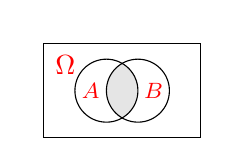
\begin{tikzpicture}[xscale=0.4, yscale=0.4]
	\fill[white, fill opacity=0] (-0.5,0) rectangle (5, 3.5); % Weisser rand um Grafik
	
	
	%\fill[white] (0,0) rectangle (5,3);
	\draw (0,0) rectangle (5,3);
	\node[red] at (0.7,2.3) {$\Omega$};
	
	\begin{scope} %Schnittmenge färben
		\clip (2,1.5) circle[radius=1];
		\fill[gray!20] (3,1.5) circle[radius=1];
	\end{scope}
	
	\draw (2,1.5) circle[radius=1]; %Kreise Zeichnen
	\draw (3,1.5) circle[radius=1];
	
	\node[red] at (1.5, 1.5) {\footnotesize$A$};
	\node[red] at (3.5, 1.5) {\footnotesize$B$};
	
	%\draw[help lines] (0,0) grid (5,3);
\end{tikzpicture}
 & $A \cap B$\\
		\hline
		$A$ oder $B$ & Vereinigung & %Autor: Simon Walker
%Version: 1.0
%Datum: 25.11.2019
%Lizenz: CC BY-NC-SA

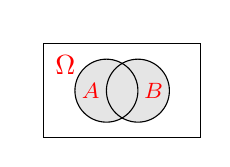
\begin{tikzpicture}[xscale=0.4, yscale=0.4]
	\fill[white, fill opacity=0] (-0.5,0) rectangle (5, 3.5); % Weisser rand um Grafik
	
	%\fill[white] (0,0) rectangle (5,3);
	\draw (0,0) rectangle (5,3);
	\node[red] at (0.7,2.3) {$\Omega$};
	
	\fill[gray!20] (2,1.5) circle[radius=1]; %Fläche färben
	\fill[gray!20] (3,1.5) circle[radius=1];
	
	\draw (2,1.5) circle[radius=1]; %Kreise Zeichnen
	\draw (3,1.5) circle[radius=1];
	
	\node[red] at (1.5, 1.5) {\footnotesize$A$};
	\node[red] at (3.5, 1.5) {\footnotesize$B$};
	
	%\draw[help lines] (0,0) grid (5,3);
\end{tikzpicture}
 & $A \cup B$\\
		\hline
		$A$ hat $B$ zur folge & A ist in B enthalten & %Autor: Simon Walker
%Version: 1.0
%Datum: 25.11.2019
%Lizenz: CC BY-NC-SA

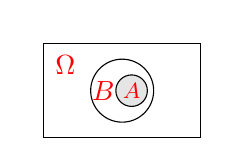
\begin{tikzpicture}[xscale=0.4, yscale=0.4]
	\fill[white, fill opacity=0] (-0.5,0) rectangle (5, 3.5); % Weisser rand um Grafik
	
	%\fill[white] (0,0) rectangle (5,3);
	\draw (0,0) rectangle (5,3);
	\node[red] at (0.7,2.3) {$\Omega$};
	
	\fill[white] (2.5, 1.5) circle [radius=1];
	\draw (2.5,1.5) circle [radius=1];
	\node[red] at (1.9, 1.5) {$B$};
	
	\fill[gray!20] (2.8, 1.5) circle [radius=0.5];
	\draw (2.8,1.5) circle [radius=0.5];
	\node[red] at (2.8, 1.5) {\footnotesize $A$};
	
	
	%\draw[help lines] (0,0) grid (5,3);
\end{tikzpicture}
 & $A \subset B$ \\
		\hline
		nicht $A$ & Komplementär Ereignis & %Autor: Simon Walker
%Version: 1.0
%Datum: 25.11.2019
%Lizenz: CC BY-NC-SA

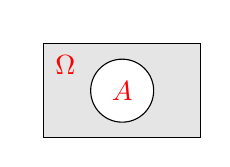
\begin{tikzpicture}[xscale=0.4, yscale=0.4]
	\fill[white, fill opacity=0] (-0.5,0) rectangle (5, 3.5); % Weisser rand um Grafik
		
	\fill[gray!20] (0,0) rectangle (5,3);
	\draw (0,0) rectangle (5,3);
	\node[red] at (0.7,2.3) {$\Omega$};
	
	\fill[white] (2.5, 1.5) circle [radius=1];
	\draw (2.5,1.5) circle [radius=1];
	
	\node[red] at (2.5, 1.5) {$A$};
	
	%\draw[help lines] (0,0) grid (5,3);
\end{tikzpicture}
 & $\Omega\setminus A$\\
		\hline
	\end{tabular}
\vspace{.2cm}
\hrule

\subsection{Wahrscheinlichkeit \& Rechenregeln}
	\begin{tabular}{l:l}
	  Wertebereich: & ${0}\le{P(A)}\le{1}$\\ \hdashline
	  Sicheres Ereignis:    & $P(\Omega)=1$\\ \hdashline
	  unmögliches Ereignis: & $P(\emptyset)=0$\\ \hdashline
	  komplementär Ereignis: & $P(\bar{A})=P({\Omega}\setminus{A})=1-P(A)$\\ \hdashline
	  Differenz der Ereignisse A und B: & $P({A}\setminus{B})=P(A)-P({A}\cap{B})$\\ \hdashline
	  Vereinigung zweier Ereignisse: & $P({A}\cup{B})=P(A)+P(B)-P({A}\cap{B})$\\
	\end{tabular}
	
	\[P(A)=\lim\limits_{\text{Anzahl Versuche} \to \infty} \dfrac{\text{Anzahl Versuche bei der A eingetreten ist}}{\text{Anzahl Versuche}}
	\]
\vspace{.2cm}
\hrule

\subsection{Laplace-Experiment}
	In einem endlichen Wahrscheinlichkeitsraum $\Omega$ haben alle
	Elementarereignisse die gleiche Wahrscheinlichkeit.\\[2pt]
	$\boxed{P(A)=\dfrac{\left| A\right|}{\left|\Omega\right|}}$\\[2pt]
	\textbf{Beispiele:} Münzen werfen wenn der Rand vernachlässigt wird, Würfeln... 
\vspace{.2cm}
\hrule


\subsection{Bedingte Wahrscheinlichkeit}
	Die Wahrscheinlichkeit für das Eintreten des Ereignisses $A$ unter der
	Bedingung, dass das Ereignis $B$ bereits eingetreten ist.\\[.2cm]
	$\boxed{P(A\mid B)= \dfrac{P(A\cap B)}{P(B)}}=\underbrace{\frac{P(A)\cdot
	  P(B)}{P(B)}=P(A)}_{\text{nur wenn unabhängig}}$ \\
		$P(\overline{A}|B) = 1 -
	  P(A|B)$
\vspace{.2cm}
\hrule

\subsection{Unabhängige Ereignise}
	Für sie gilt \hspace*{5mm} $\boxed{P(A\cap B)=P(A)P(B)}$\\[2pt]
   	Die Tatsache, dass A eingetreten ist, hat keinen Einfluss auf die 
	Wahrscheinlichkeit von B.\\
	Unabhängige Ereignisse $A$ und $B$ liegen vor, wenn: 
	\hspace*{5mm} $P(A\mid B)=P(A\mid \overline{B})$ \\	
	Wenn Ereignisse nicht gleichzeitig eintreten können, so sind sie abhängig.\\
	%Autor: Simon Walker
%Version: 1.0
%Datum: 30.11.2019
%Lizenz: CC BY-NC-SA

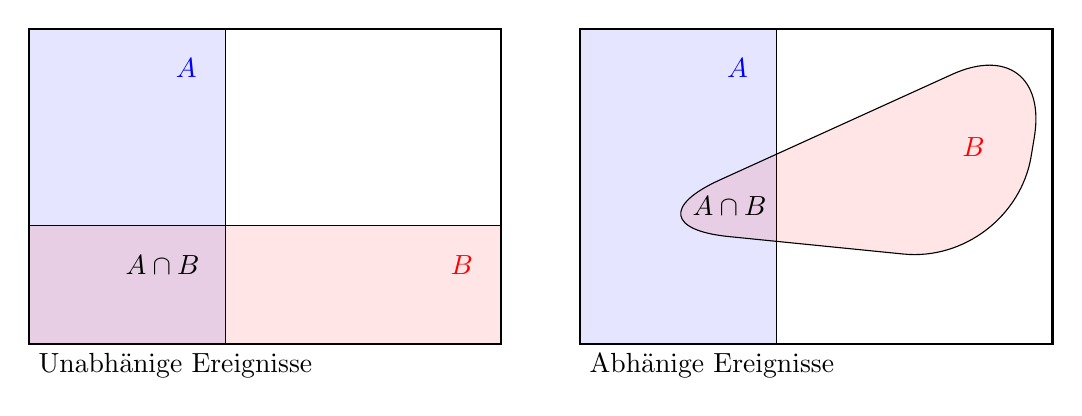
\begin{tikzpicture}

%	\newcommand{\HelpCords}[4]{
%		\draw [help lines] (#1,#2) grid (#3,#4);
%		\foreach \i in {#1,..., #3}
%		\node [below] at (\i,#2) {$\i$};
%		\foreach \i in {#2,..., #4}
%		\node [left] at (#1,\i) {$\i$};
%	}

	\filldraw [draw=black, fill=blue, fill opacity=.1] (0,0) rectangle (2.5,4);
	\filldraw [draw=black, fill=red, fill opacity=.1] (0,0) rectangle (6,1.5);
	\draw [thick] (0,0) rectangle (6,4);
	\node[blue] at (2, 3.5) {$A$};
	\node[red] at (5.5, 1) {$B$};
	\node at (1.7, 1) {$A\cap B$};
	\node[below right] at (0,0) {Unabhänige Ereignisse};
	
	
	\filldraw [draw=black, fill=blue, fill opacity=.1] 
	(7,0) rectangle (9.5,4);
	\filldraw [draw=black, fill=red, fill opacity=.1, rounded corners=14mm, smooth] 
	(13,4) -- (7.5, 1.5) -- (12.5, 1) -- cycle;
	\draw [thick] (7,0) rectangle (13,4);
	\node[blue] at (9, 3.5) {$A$};
	\node[red] at (12, 2.5) {$B$};
	\node at (8.9, 1.75) {$A\cap B$};
	\node[below right] at (7,0) {Abhänige Ereignisse};
	
%	\HelpCords{0}{0}{6}{4}
%	\HelpCords{7}{0}{13}{4}
	
	
\end{tikzpicture}\\
	Beim Beispiel mit abhängigen Ereignissen wird $A$ unwahrscheinlicher, wenn bereits $B$ eingetroffen ist.  
\vspace{.2cm}
\hrule

\begin{minipage}[t]{0.6\textwidth}
	\vspace{2mm}
	\subsection{Totale Wahrscheinlichkeit}
		$\boxed{P(A)=\sum\limits_{i=1}^n P(A\mid B_i)\cdot P(B_i)}$ \\
	
		in Matrixform: \\
		$\begin{pmatrix}P(A_1)\\P(A_2)\\\vdots\\P(A_n)\end{pmatrix} = 
		\underbrace{\begin{pmatrix}P(A_1|B_1) & P(A_1|B_2) & \ldots & P(A_1|B_n) \\
		P(A_2|B_1) & P(A_2|B_2) & \ldots & P(A_2|B_n) \\
		\vdots & \vdots & \ddots & \cdots \\
		P(A_m|B_1) & P(A_m|B_2) & \ldots & P(A_m|B_n)\end{pmatrix}}_{\text{W'keitsmatrix}}
		\cdot \begin{pmatrix}P(B_1)\\P(B_2)\\\vdots\\P(B_n)\end{pmatrix}$
		\vspace{.2cm}
\end{minipage} \hspace{0.05\textwidth} \vrule \hspace{0.05\textwidth}
\begin{minipage}[t]{0.3\textwidth}
	\vspace{2mm}
	\subsection{Satz von Bayes}
	$\boxed{P(B\mid A)=P(A\mid B) \cdot\dfrac{P(B)}{P(A)}}$\\[2pt]
	Tauscht die Ereignisse der Bedingten Wahrscheinlichkeit. 
	\vspace{.2cm}
\end{minipage}
\hrule

\subsection{Google Matrix}
	Es gibt folgende Ereignisse: $P(S_i)=$\{Ein User ist auf der Seite i\} und \\
	\hspace*{43.3mm}$P(S_j')=$\{Ein User ist nach einem Klick auf der Seite j\} \\
	nach einiger Zeit ergibt sich ein Gleichgewicht $P(S_i)=P(S_j')$ \\
	$P(S_j')=P(S_j'|S_1)P(S_1)+P(S_j'|S_2)P(S_2)+\dots$ \\
	$\begin{pmatrix}P(S_1')\\P(S_2')\\\vdots\end{pmatrix} = 
	\underbrace{\begin{pmatrix}P(S_1'|S_1)P(S_1) & P(S_1'|S_2)P(S_2) & \ldots \\
	P(S_2'|S_1)P(S_1) & P(S_2'|S_2)P(S_2) & \ldots \\
	\vdots & \vdots & \vdots \\
	\end{pmatrix}}_{\text{H}}
	\underbrace{\begin{pmatrix}P(S_1)\\P(S_2)\\\vdots\end{pmatrix}}_{\text{p (Pagerank)}} \rightarrow Hp=p$ \\
	Wird der freie Wille noch einberechnet, dann gilt: $H'=\alpha H+\frac{1-\alpha}{\textbf{Anzahl Seiten}}A$ wobei A nur aus 1en besteht.\\
	
\hrule
